%%
%% This is file `sample-manuscript.tex',
%% generated with the docstrip utility.
%%
%% The original source files were:
%%
%% samples.dtx  (with options: `manuscript')
%% 
%% IMPORTANT NOTICE:
%% 
%% For the copyright see the source file.
%% 
%% Any modified versions of this file must be renamed
%% with new filenames distinct from sample-manuscript.tex.
%% 
%% For distribution of the original source see the terms
%% for copying and modification in the file samples.dtx.
%% 
%% This generated file may be distributed as long as the
%% original source files, as listed above, are part of the
%% same distribution. (The sources need not necessarily be
%% in the same archive or directory.)
%%
%%
%% Commands for TeXCount
%TC:macro \cite [option:text,text]
%TC:macro \citep [option:text,text]
%TC:macro \citet [option:text,text]
%TC:envir table 0 1
%TC:envir table* 0 1
%TC:envir tabular [ignore] word
%TC:envir displaymath 0 word
%TC:envir math 0 word
%TC:envir comment 0 0
%%
%%
%% The first command in your LaTeX source must be the \documentclass command.
\documentclass[manuscript,screen,review]{acmart}

%%
%% \BibTeX command to typeset BibTeX logo in the docs
\AtBeginDocument{%
  \providecommand\BibTeX{{%
    Bib\TeX}}}

%% Rights management information.  This information is sent to you
%% when you complete the rights form.  These commands have SAMPLE
%% values in them; it is your responsibility as an author to replace
%% the commands and values with those provided to you when you
%% complete the rights form.
\setcopyright{acmcopyright}
\copyrightyear{2022}
\acmYear{2022}
\acmDOI{XXXXXXX.XXXXXXX}

%% These commands are for a PROCEEDINGS abstract or paper.
%\acmConference[Conference acronym 'XX]{Make sure to enter the correct
 % conference title from your rights confirmation emai}{June 03--05,
 % 2018}{Woodstock, NY}
%\acmPrice{15.00}
%\acmISBN{978-1-4503-XXXX-X/18/06}


%%
%% Submission ID.
%% Use this when submitting an article to a sponsored event. You'll
%% receive a unique submission ID from the organizers
%% of the event, and this ID should be used as the parameter to this command.
%%\acmSubmissionID{123-A56-BU3}

%%
%% For managing citations, it is recommended to use bibliography
%% files in BibTeX format.
%%
%% You can then either use BibTeX with the ACM-Reference-Format style,
%% or BibLaTeX with the acmnumeric or acmauthoryear sytles, that include
%% support for advanced citation of software artefact from the
%% biblatex-software package, also separately available on CTAN.
%%
%% Look at the sample-*-biblatex.tex files for templates showcasing
%% the biblatex styles.
%%

%%
%% The majority of ACM publications use numbered citations and
%% references.  The command \citestyle{authoryear} switches to the
%% "author year" style.
%%
%% If you are preparing content for an event
%% sponsored by ACM SIGGRAPH, you must use the "author year" style of
%% citations and references.
%% Uncommenting
%% the next command will enable that style.
%%\citestyle{acmauthoryear}


\usepackage{wrapfig}

%%
%% end of the preamble, start of the body of the document source.
\begin{document}

%%
%% The "title" command has an optional parameter,
%% allowing the author to define a "short title" to be used in page headers.
\title{Scaling ML Training: A priori estimates on data and system requirements for scaling ML training tasks}

%%
%% The "author" command and its associated commands are used to define
%% the authors and their affiliations.
%% Of note is the shared affiliation of the first two authors, and the
%% "authornote" and "authornotemark" commands
%% used to denote shared contribution to the research.
\author{Aaron D. Saxton}
\authornote{Both authors contributed equally to this research.}
\email{saxton@illinois.edu}
\orcid{1234-5678-9012}
\affiliation{%
  \institution{UIUC: NCSA}
  \streetaddress{}
  \city{Urbana}
  \state{Illinois}
  \country{USA}
  \postcode{61820}
}



%%
%% By default, the full list of authors will be used in the page
%% headers. Often, this list is too long, and will overlap
%% other information printed in the page headers. This command allows
%% the author to define a more concise list
%% of authors' names for this purpose.
\renewcommand{\shortauthors}{Saxton et al.}

%%
%% The abstract is a short summary of the work to be presented in the
%% article.
\begin{abstract}


One paper that could be "low hanging fruit" is discussing data availability for training and studying models at large, HPC, scale. The sections would be,
Introduction talk about sterile bench marking of training. In particular, how ResNet50 is trained from scratch on ImageNet data.
Point out the data is heavily curated and the expected generalization gap is well known.
Show benchmarks involving the volume of data that needs to be hosted and processed
Validating an unstudied model.
Types of validation
explain-ability
types of data operations needed to curate data and build appropriate validation
Application to broad categories of models. Curating and meaningful validation. Data volume and throughput requirements for each of these.
Static graph CNN's
Auto encoding and clustering
Sequence models.
\end{abstract}

%%
%% The code below is generated by the tool at http://dl.acm.org/ccs.cfm.
%% Please copy and paste the code instead of the example below.
%%
\begin{CCSXML}
<ccs2012>
 <concept>
  <concept_id>10010520.10010553.10010562</concept_id>
  <concept_desc>Computer systems organization~Embedded systems</concept_desc>
  <concept_significance>500</concept_significance>
 </concept>
 <concept>
  <concept_id>10010520.10010575.10010755</concept_id>
  <concept_desc>Computer systems organization~Redundancy</concept_desc>
  <concept_significance>300</concept_significance>
 </concept>
 <concept>
  <concept_id>10010520.10010553.10010554</concept_id>
  <concept_desc>Computer systems organization~Robotics</concept_desc>
  <concept_significance>100</concept_significance>
 </concept>
 <concept>
  <concept_id>10003033.10003083.10003095</concept_id>
  <concept_desc>Networks~Network reliability</concept_desc>
  <concept_significance>100</concept_significance>
 </concept>
</ccs2012>
\end{CCSXML}

\ccsdesc[500]{Computer systems organization~Embedded systems}
%\ccsdesc[300]{Computer systems organization~Redundancy}
%\ccsdesc{Computer systems organization~Robotics}
%\ccsdesc[100]{Networks~Network reliability}

%%
%% Keywords. The author(s) should pick words that accurately describe
%% the work being presented. Separate the keywords with commas.
\keywords{datasets, neural networks, model training at scale}

%%
%% This command processes the author and affiliation and title
%% information and builds the first part of the formatted document.
\maketitle

%\section{Introduction}

Facilitating scientists and engineers to perform large scale modeling has been one of the strengths of HPC. Most modeling methods can be organized into one of Phillip Colella's "Seven Dwarves"

 As Phillip Colella Hardware architectures, software, and data pipelines have been executed ad nauseam with traditional approaches included in Phillip Colella's "Sevens Dwarves" problems. Some interesting features 
In this document we argue that recent modern ML methods are unique in that the size of the trainable parameters in the model is large, the data is large, and for the foreseeable future the precise details of the model and data are discovered through trial and error. This means practitioners need to balance what is in memory and what get's loaded from a file system, and during model design high levels of interactivity is necessary to facilitate serendipitous discovery.

Because ML/AI have no methods like heat eq condition, properties discovered with small amount of data and small models rarely extend to larger situations.


Holisticly looking at the entire process of studying large datasets with modern ML models.

Designing and training models from scratch.

Desired features, capacity of model.

Feature engineering.
\section{Background into Classic Methods}



Features in data are often colloquially spoken of but rarely have rigorous descriptions. We will look at a common dataset to illustrate how features express them selves: The "Iris Dataset"\cite{Iris:Fisher} . This dataset is an excellent playground to bridge the gap between statistical intuition and formal analysis on higher dimensional data. The Iris flower has been formally studied by botanists since 1913.The successful husbandry of these flowers are highly dependent on which species are in the genetic pool a botanist is drawing from. In Fishers 1934 paper "The use of multiple measurements in taxonomic problems" \cite{Iris:Fisher} it was surprising to observe a third species in what was previously thought to be a two species data set. This dataset was created by selecting 50 samples of flowers from each of the three species sets Setosa, Versicolor, and Virginica. With each sample, four properties were measured. The final makeup of the data set is 150 samples with 5 properties: petal length, petal width, sepal length, sepal width, and species. In the following description we will see that the species can be made dependent on the other 4 properties. 

\begin{wrapfigure}{r}{0.4\textwidth}
\centering
    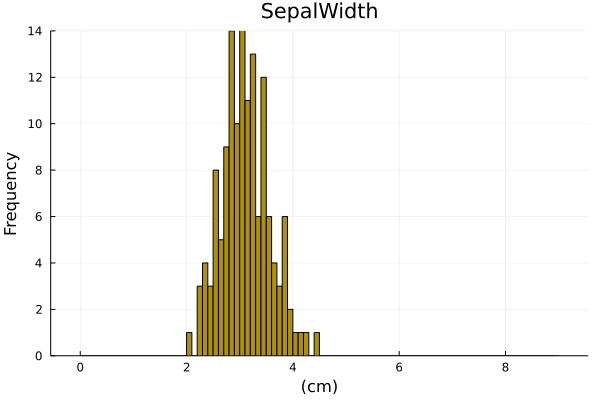
\includegraphics[width=0.35\textwidth]{Code/SepalWidthTotHist.png}
    \caption{Histogram of sepal width from the Iris dataset}
    \label{fig:SepalWidthTotHist}
\end{wrapfigure}
Distributions and histograms are ubiquitous in any scientific analysis, but for emphasis it bears repeating here. A \emph{histogram} is constructed by counting the frequency a property in a dataset obtains a certain value (or range of values). For example in Fig. \ref{fig:SepalWidthTotHist}. the property sepal width is binned into bins of 1 mm width between 0 and 9 cm. The histogram tells us that sepal width is roughly between 2cm and 5cm with a large concentration at about 3 cm. Finally, one may also observe that the histogram is roughly the shape of a bell curve. These are interesting qualitative features to observe, but more importantly, this histogram, after normalizing, is an approximation to a \emph{probability distribution}. In a subject matter specific setting, exactly the distribution that this data is drawn from would be hotly contested based on expert testimony of what could be driving the variation.
\begin{wrapfigure}{l}{0.4\textwidth}
\centering
    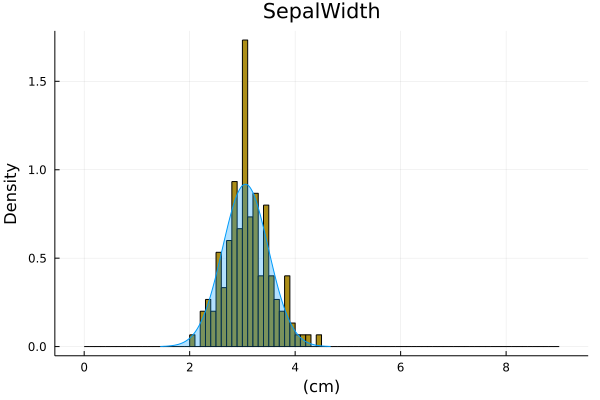
\includegraphics[width=0.35\textwidth]{Code/SepalWidthTotHistFit.png}
    \caption{Normalized histogram with fitted probability density overlay }
    \label{fig:SepalWidthTotHistFit}
\end{wrapfigure}

For demonstration purposes, assume that the physics, chemistry, and biology cause sepal width to be drawn from a normal distribution. The probability density function for a normal distribution is the Gaussian function. After normalization, the gaussian can be parameterized by two values: The \emph{mean}, which is also called the \emph{expected value}, and the \emph{variance} which is related to the \emph{standard deviation}. In Fig. \ref{fig:SepalWidthTotHistFit} a normal distribution has been fit to the sepal width and overlayed on top of the normalized histogram. While this example may be overly pedantic, \textbf{it is important to note that the algorithm to fit a single gaussian is brute force arithmetic of computing the mean and variance}. The fitted normal distribution gives a model by which to compare and measure new data against. So far the sepal width data has not given any profound insights. At most, if a graduate student was sent to the green houses to measure flowers and they came back with many samples of lengths around 6cm, you could compute the \emph{log likelihood} and quantitatively see that the graduate student did not know the difference between an Iris and, say, a Lili. The usefulness of this model is marginal. However, all is not lost, there are still 3 more properties to analyze and extract meaningful insight.
\begin{figure}[h]
\centering
    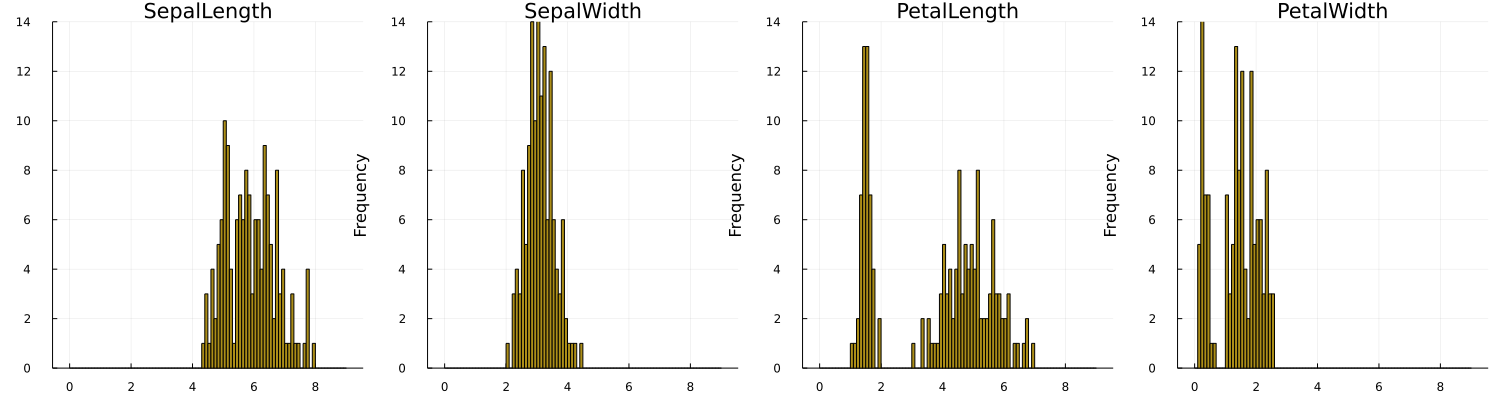
\includegraphics[width=1.0\textwidth]{Code/propHist4x1_tot.png}
    \caption{Histograms of each of the 4 properties measured in the Iris dataset }
    \label{fig:propHist4x1_tot}
\end{figure}
Let us examine the histograms of all properties in Fig. \ref{fig:propHist4x1_tot}. If one tries to fit a Gaussian function to the remaining properties, the error from sepal length will be modest, however the error from fitting gaussian to petal length or petal width will be significantly more. Or in other words, a normal distribution is a bad model for petal length and petal width. A blind approach to find a good model would be to try popular classic distribution like a beta, gamma, or exponential  distribution. Unfortunately, these will suffer from the same bad error that a normal distribution did. More exotic models are required. There is no full-proof standard way of choosing an optimal model \footnote{If we made assumptions about the underlying causality of what is driving this data we could indeed choose a class of models or even a specific parameterized model}. As uncomfortable as it may be, this is where science becomes an art, and also the root of why it is so hard to define an abstract and formal definition of a \emph{feature in data}. Many human brains may look at the petal length and width histograms and see two vague curves in each. This is inspiration enough to choose a Gaussian Mixture Model (GMM). 


\begin{wrapfigure}{l}{0.5\textwidth}
\centering
    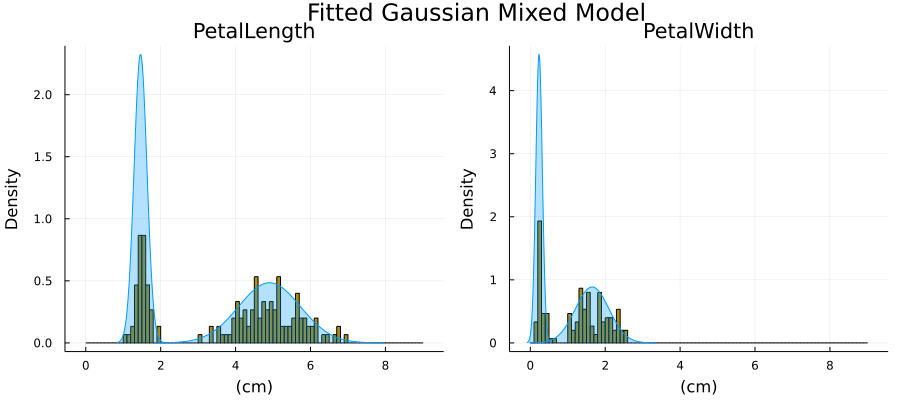
\includegraphics[width=0.5\textwidth]{Code/propHist2x1_OverTot.png}
    \caption{EM optimization initialized with means of 0, 5 and variance of 0.01, 0.1}
    \label{fig:propHist2x1_OverTot}
\end{wrapfigure}
There are many details to choosing and fitting the right GMM. In this case, there are three important details to explore. First, the mixture will contain two normal distributions. That means it is parameterized by a total of four parameters, two means and two variances. But, unlike a single normal distribution, computing the mean and variances to fit the model requires a more delicate approach. Second, It might feel like cheating for a human to choose a parameterized class of models (in this case, a two mode GMM), it is certainly cheating for a human to choose which subset of data they wish to compute the means and variances. Instead, the algorithm to fit the distribution using the entire dataset will be \emph{expectation maximization} (EM)\footnote{EM is considered a classic statistical leaning method. Because of its iterative nature, its spirit is very similar to more recent machine learning models and stochastic gradient decent.}.
\begin{wrapfigure}{r}{0.35\textwidth}
\centering
    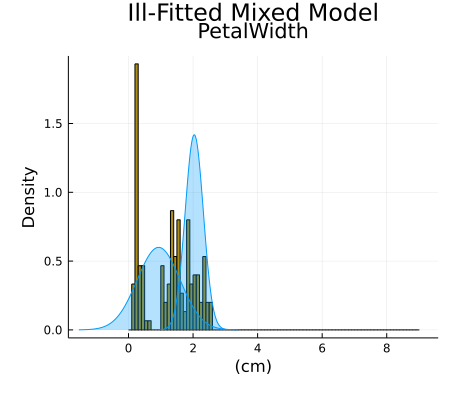
\includegraphics[width=0.35\textwidth]{Code/propHist2x1_OverTot_bad.png}
    \caption{EM optimization initialized with means of 0, 5 and variance of 0.1, 0.1. Resulted in poor fitting }
    \label{fig:propHist2x1_OverTot_bad}
\end{wrapfigure}
This algorithm can be roughly thought of as an iterative gradient method for optimizing the distributions parameters to achieve a best fit. Third, the EM algorithm can be very sensitive to the models initial parameters. Especially in one property dimension. Compare the difference between Fig. \ref{fig:propHist2x1_OverTot} and Fig. \ref{fig:propHist2x1_OverTot_bad}. With only a modest change in variance results in a reasonable fit in Fig. \ref{fig:propHist2x1_OverTot} and an absurd fit in Fig. \ref{fig:propHist2x1_OverTot_bad}.

In Fig. \ref{fig:propHist2x1_OverTot} there are acceptable fitted models to describe petal length and width. Petal length, qualitatively, has the more separated gaussian means between each lobe, let's focus on this property to identify the major object of interest, \emph{features in data}. Features in data are properties that can be measured. The goal of fitting an explicit model to the data is to create unambiguous values to make a measure against. To this end the fitted mixed models gives us explicit values for the means and variances of two Gaussians. We define features of this data with its model by measuring which gaussian each sample of data belongs to. Given a single example and using the formula for a gaussian, this can be done by computing the probability with respect to each gaussian. A feature will be assigned based on whichever probability is higher. Qualitatively, \emph{features in data} are subsets of data that can be "bunched together". Formally and abstractly, a feature in data is a subset that can be measured against some stochastic process like the example described above.

\begin{figure}[h]
\centering
    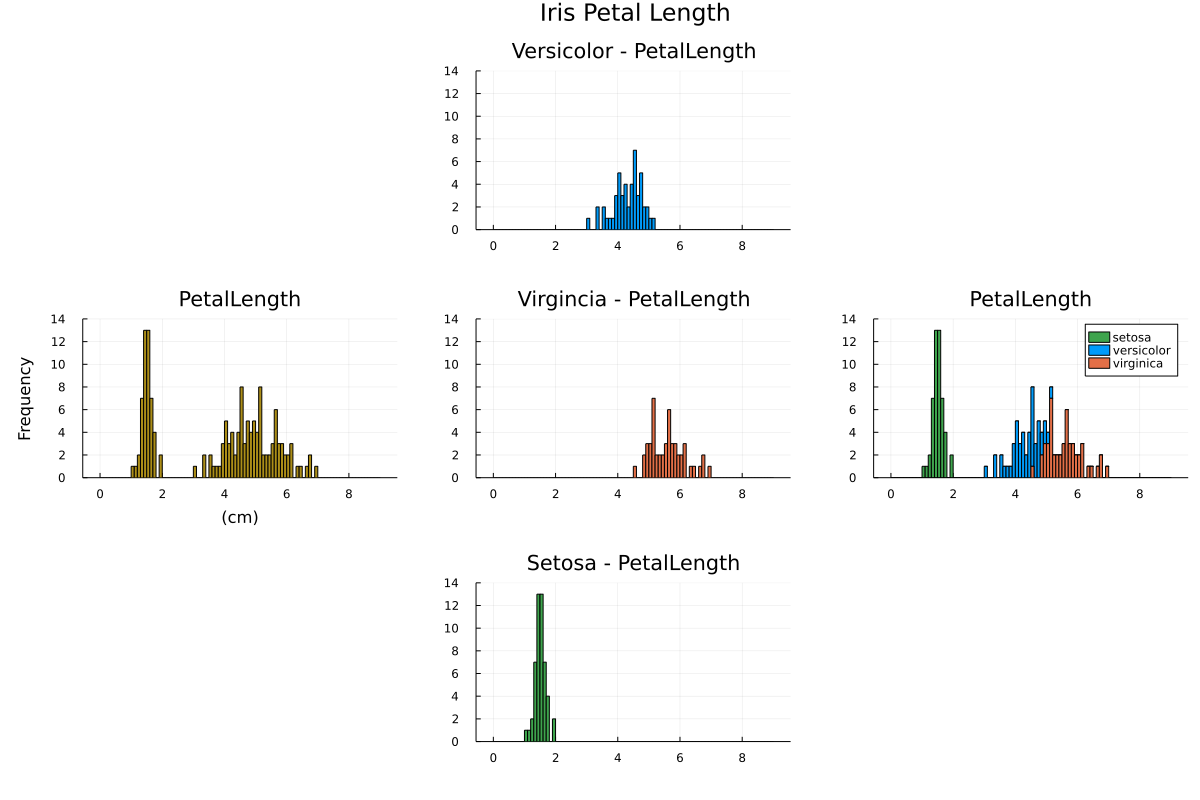
\includegraphics[width=1.0\textwidth]{Code/histBreakoutPetalLength.png}
    \caption{Breakout histograms of species }
    \label{fig:specBreakout}
\end{figure}

So far in this discusion, the features have no connection to reality. It is merely a curiosity that the data set has two statistically interesting features. This may lead one to perform further analysis of these samples. Indeed, in Fisher's paper \cite{Iris:Fisher} he describes that a mixture of husbandry practices and what are now known as early forms of genetic testing identify each sample with their genetic species. In figure Fig. \ref{fig:specBreakout} we reveal that the features in data that was discovered with the gaussian mixed model correspond to the Iris species Setosa in one feature, then versicolor and virginica in the second feature. It is important to note that in reality the genetics of the species causes, or implies, the length of petal. This discussion, however, focused on and found features in the data first, without having knowledge of the species, that can be used to guide further investigation by subject matter experts. This is the power of identifying features in data. The process of labeling data and finding features in data goes both ways.

The gaussian mixed model was able to isolate Setosa Iris as a feature. Even though the model was limited to 2 gaussians Fig. ref{fig:specBreakout} makes it clear that if a third was added the second and third gaussian would have struggle to fit the remaining species. This is a good opportunity to introduce join probability distributions and observe the importance of dimensionality. Features in data is also a story about dimensionality. A famous result in knot theory is "You can't tie your shoes in 4 dimensions". This is tragic for any aspiring high dimensional athletes, but good news for data scientists. 
\begin{wrapfigure}{l}{0.60\textwidth}
\centering
    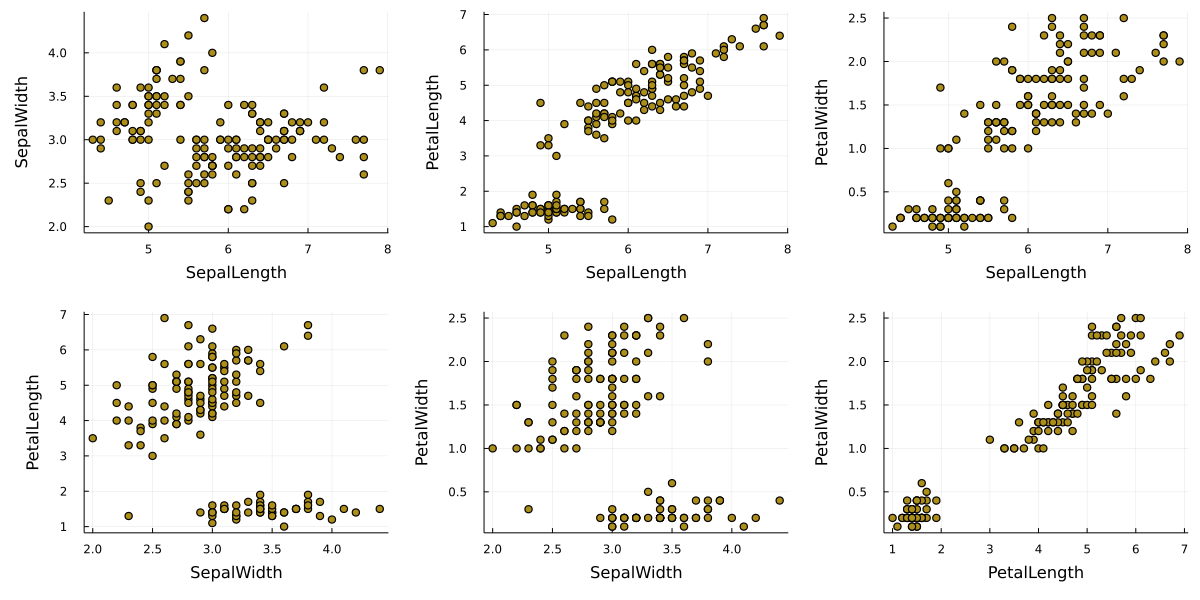
\includegraphics[width=0.60\textwidth]{Code/3by2PropVsPropUnLabeled.png}
    \caption{Estimations of join probability distribution of each pair of Iris properties}
    \label{fig:3by2PropVsPropUnLabeled}
\end{wrapfigure}
\begin{wrapfigure}{r}{0.60\textwidth}
\centering
    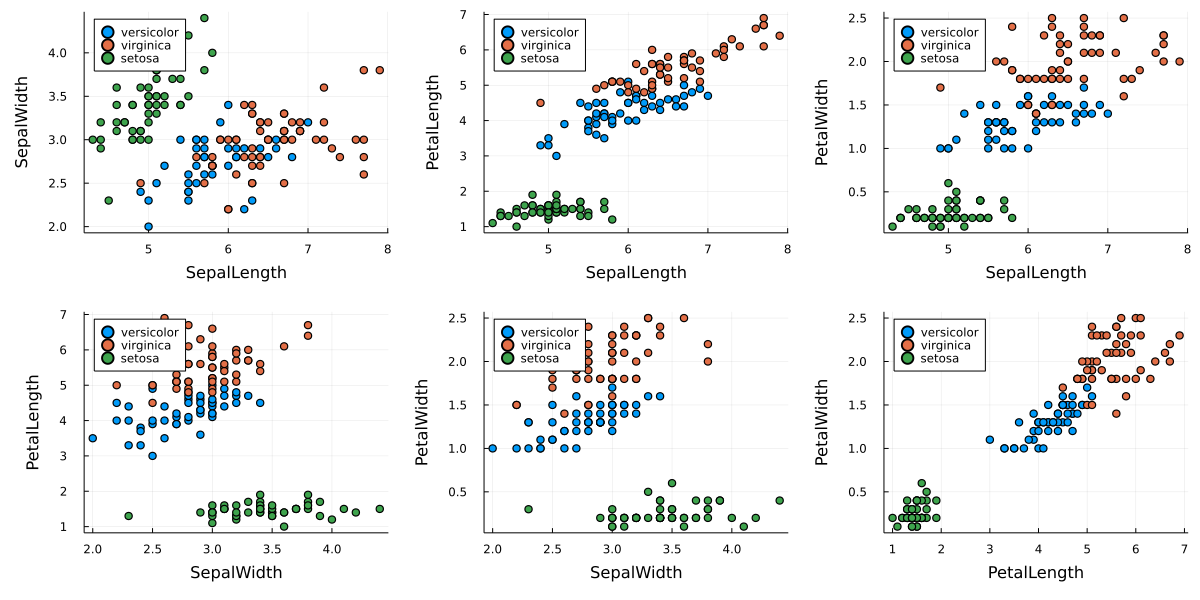
\includegraphics[width=0.60\textwidth]{Code/3by2PropVsPropLabeled.png}
    \caption{Estimations of join probability distribution of each pair of Iris properties}
    \label{fig:3by2PropVsPropLabeled}
\end{wrapfigure}
\emph{Joint probability distributions} in two properties is a function with two independent input variables and an output of a probability density for each pair of inputs. The scatterplots in Fig. \ref{fig:3by2PropVsPropUnLabeled} is not exactly a histogram or distribution. However, by partitioning the two dimensional domain into bins and counting the samples that are in each bin, one could imagine how these scatter plots represent an approximation to a distribution. It is important to note that the two dimensional domain is not as "full" as the one dimension domain. That is, if the domains were binned with, say, 1mm bins, the number of occupied bins is proportionally less in two dimensions than in one. \textbf{To properly sample higher dimensional spaces requires $O(p^n)$ more samples}. One can also observe samples bunching together creating areas of higher density.  The lessons learned from the one dimensional gaussian mixed model can be applied here, albeit with more parameters. Indeed, a multivariate normal distribution is parameterized by a \emph{mean} and \emph{variance} but the mean will be a $1 \times n$ vector and the variance will be a $n \times n$ matrix. Each item in the mean vector will be the simple mean that corresponds with its positions variable, but the variance matrix is made up of the variance and covariance of every variable measured agains every other variable. It is beyond the scope of this manuscript to go into depth about the specific meaning of these parameters, but the message that should be leaned here is \textbf{as dimensionality increases, so does the parameters in the models}. In this case, parameters grow as $n^2$. Also, the size of the model will grow linearly with number of features that are expected in the data. With this lesson in mind, we will forego the formal fitting of a model and just accept it'll be much bigger than the one dimensional case. In the Petal Width vs. Petal Length plot of Fig. \ref{fig:3by2PropVsPropUnLabeled} one can observe that there is a clear dense cluster in the lower left hand corer. Furthermore, squinting at the other cluster, one may be able to make out there are two dense centers. Formally fitting a three Gaussian mixed model distribution would reveal this also. Indeed, Fig. \ref{fig:3by2PropVsPropLabeled} shows that these cluster are species. Dimensionality does have its limits. Performing this same kind of analysis on 4 property dimensions will give a more certain model, a model that gives confidence that this dataset contained 3 species and not just two, it will never be a perfect predictor to distinguish between Versicolor and Virgincia Iris \cite{Iris:Fisher}. However it is good enough to select varieties to breed an award winning Iris garden.

Before this section ends, it is important to point out the limitations of leveraging higher dimensional property spaces to build better models. Higher dimensional spaces are inherently harder to analyze. We appeal to information theory, in particular Shannons information measures, to bridge the gap between a rigorous approach and a usable intuition of what data can still benefit from higher dimensions.

As seen above, the information encoded in the 4d data can be segmented into features, but the features themselves can be encoded as a fifth property of each sample. That is, as the species label. The fitted distribution combined with measuring features in data makes up a model that takes an input vector and assigns a feature label as an output. In a good dataset, there is a one-to-one correspondence between how features are encoded in certain properties and a feature label in an additional property.

Shannons information measure


\section{Current Modern Models}
\begin{wrapfigure}{l}{0.4\textwidth}
\centering
    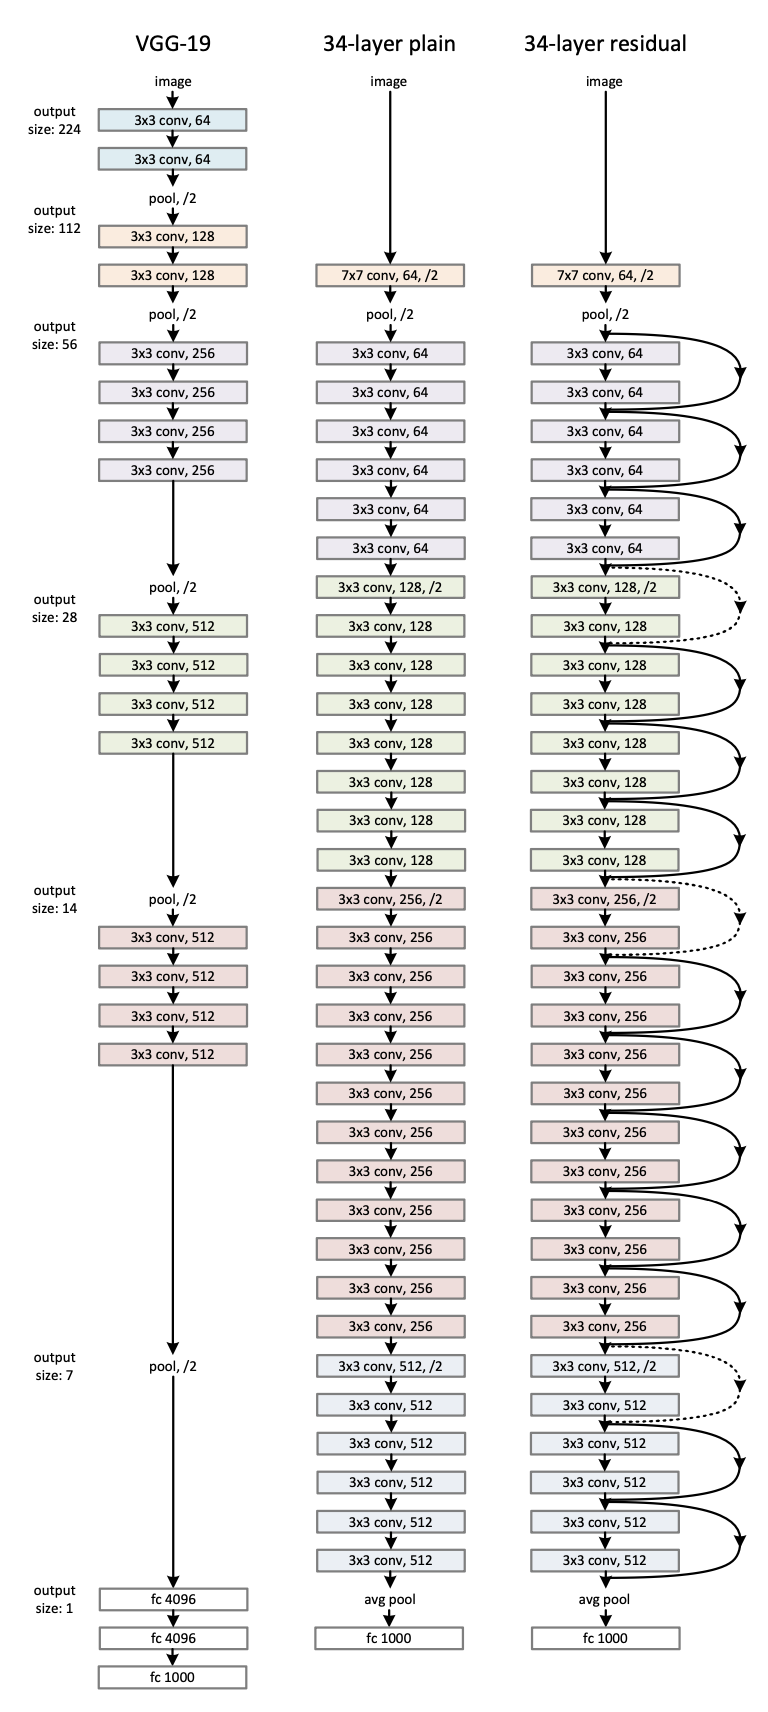
\includegraphics[width=0.35\textwidth]{ResNet50Graph.png}
    \caption{Block Diagram of VGG-19, Precursor to ResNet, and ResNet-34 \cite{ResNet50:He}}
    \label{fig:ResNet50Graph}
\end{wrapfigure}
In the previous section we observed a scaling property of model size as it relates to number dimensions of the data, $O(n^2)$. Also the model would scale as $O(k)$ for $k$ features Many modern problems operate on images data, which abstractly is very high dimensional data. A model would take an image as an input and returns the feature of that image as a classification. That is, the model would return if an image contains a boat or a cat. Even analyzing sets of small images will cause traditional models to be uncomputable. For example a small preview image may be 150 by 150 pixels in 3 channels which gives 67.5k dimensions. A classic model would need about 4.5B parameters. Aside from this many parameters pushing the limits of computing machines, there are classic abstract reasons parameterizing a distribution of this size is intractable and would only be used in the most exotic circumstances. This is where modern Machine Learning (ML) enters the picture. It is beyond the scope of this document to heuristically explore the development of ML from first principles in a way we did with the Iris dataset. Instead we explore one of the more recent and successful models developed, ResNet50 \cite{ResNet50:He}. ResNet50 has about 23M trainable parameters which is 3 orders of magnitude less than the modest estimate above for a classic approach. Just as the Gaussians in the  GMM had a distinct formula, so does ResNet50. It was intentional that the formula for the Gaussian, while beautiful, was never written in this document. Writing the explicit formula that makes up ResNet50 would be terse and offers no additional insight. Instead, very large models are often made up of many repeating part. ResNet50 is made of convolutions, neural networks, residuals, and batch norms. Block diagrams offer more insight. In Fig. \ref{fig:ResNet50Graph} is the diagram of ResNet50 along with two predecessors. From it we can get a rough order of magnitude how deep it is, especially compared to an earlier model, and what might be the defining characteristic of ResNet50 compared to other models. In this case, it's arrows that bypass several blocks at a time are the unique additional feature. They are called the residual layers. One lesson learned from the fitting the GMM in the previous section was the fitting algorithm is very sensitive to how the model was initialized for EM. The effort that went into the development of ResNet50 focused on reducing trainable parameters while improving the stability of how training algorithms find optimal parameters for a model. What is more, it is believed that a model having many layers (e.g. a deep model) is the quality that allows allows training algorithms to efficiently find optimal parameters for such large dimensional data \cite{nguyen2018on} \cite{janocha2017loss}.

Next, we look closer at loss functions and how ResNet50 is trained. Let $\Theta$ be the high dimensional tensor of ResNet50 parameters. Let $M$ be the number of parameters in $\Theta$. That is, $\Theta$ is the collection of all $M=$ 23 Million parameters of ResNet50. Let $D=\{x_i, y_i\}_{i\in1,...,N}$ be the samples in a dataset where $x_i$ is the input and $y_i$ is the output e.g. the labeled features. In the Iris dataset, $x_i$ would be the 4d property vector and $y_i$ would be the species label. Let $m_\Theta(x)$ denote the model with input $x$ and parameters $\Theta$.

In order to finish the description of a loss function, all the ingredients must be able to have arithmetic performed on them. $\Theta$ is a large collection of real number. It has arithmetic defined. $\{x_i\}$ for a typical ResNet50 input are numeric (usually normalized between 0 and 1) values of pixels. It has arithmetic defined. ResNet50 is a big formula, described by Fig. \ref{fig:ResNet50Graph} that does the arithmetic between $\Theta$ and $\{x_i\}$. Unfortunately, feature labels like "Setosa" or "Car" or "Cat" are not meant to be added subtracted multiplied or divided, so what should the output of a model like this look like? The concept of a \emph{one-hot encoding}, or \emph{one-hot vector} must be used. That is, for a feature set that has $k$ many items we introduce a vector that is $k\times 1$ items long. For each coordinate in the one-hot vector, the label meaning is assigned and take on a value of 1 to indicate the feature. Using the feature labels in the Iris dataset as an example, a one-hot vector could be defined in the order "Setosa", "Virgincia", "Versicolor". If $x_i$ was labeled as "Virgincia", then  $y_i = [ 0, 1, 0 ]$. The article \emph{Multivariate Bernoulli distribution} \cite{Dai:MVBer} has a more elaborate description of what a \emph{one-hot} vector can be statistically interpreted as. Even though ResNet50 is still large and seemingly opaque, it still has a foot in statistical rigor as a map between distributions \footnote{This is a stretch, but with some more research can be made precise.}. 

Finally, a loss function is going to be made of a metric that can compare two one-hot vectors and return a single real number to indicate how close, or similar, they are. There are many popular formulas such as Root Mean Square or Log Loss. The papers \cite{nguyen2018on} and \cite{janocha2017loss} explore some of the properties of different metrics. We will simply denote the metric on one-hot vectors as $l(w_1, w_2)$. The final loss function for training ResNet50 can be written as,
$$
L_D(\Theta) = \frac{1}{N}\sum_{i=1}^N l(m_\Theta(x_i), y_i) \qquad L_D: \mathbb{R}^M \to \mathbb{R}
$$
The most important detail to take away from the formula of $L_D$ is the summation. \textbf{This sum is the source of parallelism}. Whether it is  on a single GPU or across several computing devices, the fact that addition is associative is what allows the training algorithm, gradient decent, to divide $L_D$ across multiple computing devices. The second most important detail is that the $L_D$ is a function of the models parameters $\Theta$. When training a model, $D$ is fixed and $\Theta$ is varied. The third, and final, most important detail is that the training algorithm, gradient decent, computes the gradient on $L_D$ with respect to each coordinate of $\Theta$. While $L_D$ returns a scalar value,  $\nabla L_D$ returns a vector of dimension $M$. That is $L_D : \mathbb{R}^M \to \mathbb{R}$ but $\nabla L_D: \mathbb{R}^M \to \mathbb{R}^M$. Since the gradient is distributive across addition, interprocess communication is driven mostly by sharing gradients in $\mathbb{R}^M$ between kernels, cores, or hosts. Lastly, given the learning rate $\gamma$, gradient decent updates are performed on $\Theta$ as $\Theta_{\mbox{new}} = \Theta_{\mbox{old}} + \gamma \cdot \nabla L_D(\Theta_{\mbox{old}})$
\section{Conclusion}
Now that we have all the ingredients needed from both classic and modern methods, lets draw our attention to some of the parameters we listed, $n, N, M$ and $k$. That is, dimension of input data, total number of samples, number of parameters in the model, and number of features respectively. First consider $n$ and $N$. As described in the Iris dataset, it was pointed out that as we moved from one to two dimensions it would take more samples to "fill" the same "space". This notion can be heuristically made more precise by observing the volume of a hyper cube with edge length 2. In one, two and three dimensions, its "volumes" are 2, 4, 8 respectively. The space needed to be sampled grows as $p^n$. In an unfair universe, this is the growth rate that training data set would need to grow if new properties were added in order to be sure they were getting an accurate measurement of reality. Next consider $n$, $k$ and $M$. As $n$ increases, $M$ may only increase modestly for the sole purpose of dimension reduction in early layers. If the dataset is rich with information $M$ will start to growing as $O(n^2)$. The number of features $k$ may only cause $M$ to grow as the classic case $O(k)$. However, papers like \cite{nguyen2018on} and \cite{janocha2017loss} indicate that deeper models have better training properties. Higher growth may be expected. Lastly consider $N$ and $M$. These may be the most interconnected from the other two parameters. Take for example training ResNet50 on the industry standard dataset "ImageNet". ImageNet has 14M images making up 1000 feature labels and ResNet50 is often benchmarked on 3 channel images of resolution $255 \times 255$. That is $27.3\times e^{14}$ distinct values in the training dataset compared with ResNet50 23M ($e^6$). The goal of model design is to keep number of parameters low, in the foreseeable future the size of the training data, $N\times n$, will greatly out weigh the size of the models. The heaviest data movement lift in model training will be in moving the data to where the model is being computed. Moving gradients, of size $M$ will only be a modest portion of $N\times n$.

When studying new models on new sets of data, these estimates provide worst case bounds. But examples like ResNed50 give hope that it is possible to reduce model complexity and data size to achieve desirable results. Studying computer vision has a long history. It turned out there were papers from the 80's in medical imaging \cite{fukushima1982neocognitron} that got close to the performance of modern models, but the computing resources of the time prevented further discovery. When one embarks on studying a new set of data, for example high dimensional sensor data from an accelerator experiment, with a new model, one should keep in perspective the time of development of todays most popular and successful models.

\section{In regards to TriLab Job classification effort}

Monitoring data is high dimensional data. Na\"{i}vely, it's dimensions are in types of metric counters plus time steps. Even for modern ML models, the dimensionality pushes its limits. In this project we appealed to RNNs and LSTMs.

The act of labeling a monitoring dataset is wrought IT tribal turmoil and human labor intensive to boot. This effort focused on clustering and other unsupervised methods.

Since the intrinsic information in the monitoring set is unknown, it is unclear exactly what a "good sampling" would be. With Blue Waters data, our initial semi-successful clustering ocured when training on roughly 2k jobs.

\bibliographystyle{ACM-Reference-Format}
\bibliography{acmart}
\end{document}
\endinput
%%
%% End of file `sample-manuscript.tex'.
